\clearpage
\section{Quantum Noise}

\subsection*{Introduction}\label{sec:intro}


This document describes an emission and detection system which is used to simulate the effects of quantum noise. The system is based on the transmission of coherent states as the support of information. The following section introduces some aspects about coherent states, with special focus on quantum noise.\\
\\
\\
We start by defining number states $\ket{n}$ (or Fock states), which correspond to states with perfectly fixed number of photons.
\footnote{Ulf, p.21}
Associated to those states are two operators, the creation $\hat{a}^\dagger$ and annihilation $\hat{a}$ operators, which in a simple way, remove or add one photon from a given number state.
\footnote{REFERENCE}
Their action is defined as:
$$
\hat{a} \ket{n} = \sqrt{n} \ket{n-1} \qquad \qquad
\hat{a}^\dagger \ket{n} = \sqrt{n+1} \ket{n+1}
$$
$$
\hat{n} \ket{n} = n \ket{n}
$$
in which $\hat{n} = \hat{a}^\dagger\hat{a}$ is the number operator. Therefore, number states are eigenvectors of the number operator.\\
\\
Coherent states have properties that closelly resemble classical electromagnetic waves, and are generated by single-mode lasers well above the thereshold.
\footnote{Loudon, p.190}
We can defined them, using number states in the followi\ng manner:
$$
\ket{\alpha} = e^{-\frac{|\alpha|^2}{2}} \sum_{n=0}^\infty \frac{\alpha^n}{\sqrt{n!}} \ket{n}
$$
in which $\alpha$ is the sole parameter that caracterizes it.
\footnote{(number state)Loudon, p.137}
\footnote{Loudon, p.184}
\footnote{Loudon, p.186}
In fact, if we calculate the expected number of photons with $\bra{\alpha} \hat{n} \ket{\alpha}$ we will obtain $|\alpha|^2$. The coherent state is an eigenstate of the annihilation operator, $\hat{a}\ket{\alpha} = \alpha \ket{\alpha}$.\\
\\
%
%
Using the creation and annihilation operators, we can define two quadrature operators:\footnote{Loudon, p.138, (4.3.36)}

$$
\hat{X} = \frac{1}{2} \left( \hat{a}^\dagger + \hat{a} \right)
\qquad
\qquad
\hat{Y} = \frac{i}{2} \left( \hat{a}^\dagger - \hat{a} \right)
$$
The expected value of these two operators, using a coherent state $\ket{\alpha}$ are:
$$
\braket{\hat{X}} = \textrm{Re}(\alpha) \qquad \qquad
\braket{\hat{Y}} = \textrm{Im}(\alpha)
$$
We see that the expected value of these operators give us the real and imaginary part of $\alpha$. Now, we can obtain the uncertainty of these operators, using:
$$
\textrm{Var}(\hat{X}) = \braket{\hat{X}^2} - \braket{\hat{X}}^2
$$
(VALERA A PENA GENERALIZAR A QUADRATURA?)\\
For each of these quadrature operators the variance will be:
$$
\textrm{Var}(\hat{X}) = \textrm{Var}(\hat{Y}) = \frac{1}{4}
$$
This result show us that for both quadratures, the variance of measurement is the same and independent of the value of $\alpha$.\\
%
%
%
\\
\\
---WARNING: WORK IN PROGRESS---\\
{\bf Experimental setting}\\
Given an state $\ket{\alpha}$, we can use the homodyne technique to measure the phase of this signal (S), relative to the phase of a local oscillator (LO).
This technique consists in the interference of the input signal with a local oscilator which has the same frequency as the input signal, but an overwhelming largest power.\\
Operators $X$ and $Y$ correspond to the measurement of the in-phase (X) and quadrature (Y), which will depend on the phase of the local oscillator.????
\\
%(REVER UNIDADES. O QUE SAO ESTES n? Diz que e $2(\hbar\omega/2\epsilon_0V)^{1/2})$. Como se obtem V?)
\\
{\bf Noise sources}\\
There are several sources of noise, when measuring a quadrature (QUEM DIZ ISSO?). One of them is quantum noise which is related to oscillations in the electromagnetic field.
\footnote{REFERENCIA}
Other source of noise is thermal noise which is related to the electronic operations.??????\\
\\
{\bf Quantum Noise}\\
The quantum mechanical description of homodyne detection uses quantum operators to describe the effect of each component in the system. So, we start with the operators $\hat{a}_S$ and $\hat{a}_{LO}$ corresponding to the annihilation operator for the signal and local oscillator, which we be the inputs in a beam divisor. The outputs will be $\hat{a}_3$ and $\hat{a}_4$. We will use a balanced division, therefore, we can write the output as:
$$
\hat{a}_3 = \frac{1}{\sqrt{2}} \left( \hat{a}_S + \hat{a}_{LO} \right)
\qquad
\qquad
\hat{a}_4 = \frac{1}{\sqrt{2}} \left( \hat{a}_S - \hat{a}_{LO} \right)
$$
The final output of a homodyne measurement will be proportional to the difference between the photocurrents in arm $3$ and $4$. Then
$$
I_{34} = I_3 - I_4 \sim \braket{\hat{n}_3 - \hat{n}_4}
$$
We can define an operator that describes the difference of number of photons in arm 3 and arm 4:
$$
\hat{m} = \hat{a}^\dagger_3\hat{a}_3 - \hat{a}^\dagger_4\hat{a}_4
$$
If we assume the local oscillator as the coherent state $\ket{\beta}$, then the expected value of this measurement will be:
$$
\braket{m} = 2|\alpha||\beta|\cos({\theta_\alpha - \theta_\beta})
\qquad
\qquad
\textrm{Var}(m) = |\alpha|^2 + |\beta|^2
$$
The local oscillator normally has a greater power than the signal (VER REFERENCIAS), then $|\alpha| \ll |\beta|$. If we use as unit, $2|\beta|$, then these two quantities can be simplified to:
$$
\braket{m} = |\alpha|\cos({\theta_\alpha - \theta_\beta})
\qquad
\qquad
\textrm{Var}(m) =  \approx \frac{1}{4}
$$
\footnote{Referencia indirecta: Livro: Hans, p.207}
\\
We can measure the two quadratures simultaneously. We divide the signal in two beams.
One of the beams interferes with a local oscillator and the other will interfere with another oscillator that has a phase difference of $\pi/2$ relative to the other local oscillator.\\
Experimentaly, the optical hybrid (SEE SCHEME BELLOW) will take this role of mixing the signal with the two local oscillators.\\
\\
\\
SIMULATION IMPLEMENTATION:\\
In the simulator, we can model each arm's photocurrent ($I_3$ and $I_4$) and then obtain $I_{34}$ by a simple subtraction.\\
The expected value and variance of $\hat{n}_3$ is:
$$
\braket{\hat{n}_3} = \frac{1}{2} \left( |\alpha|^2 + |\beta|^2 + 2 \cos(\phi_\alpha - \phi_\beta) \right)
\qquad
\qquad
\textrm{Var}(\hat{n}_3) = \braket{\hat{n}_3}
$$
Calculating the expected value and variance for $\hat{n}_4$, we will also obtain $\textrm{Var}(\hat{n}_4) = \braket{\hat{n}_4}$, therefore both processes can be modelled by Poisson distributions:
$$
n_i \sim \textrm{Poisson}(\braket{n_i})
$$
In the simulation, a photodiode has 2 inputs. Each input corresponds to a mean complex amplitude $\bar{\Psi}_i$. This amplitude corresponds to the power $\bar{P}_i = |\bar{\Psi}_i|^2 = \braket{n_i}P_\lambda$ in which $P_\lambda$ is the power of a single photon. What we want is the power after adding noise, $P_i = n_i P_\lambda$. To model $n_i$, we will use a gaussian aproximation of $\sqrt{n_i}$, for $n_i \gg 0$, which will give us a continuous distribution:
$$
\sqrt{n_i} \sim \textrm{Gaussian}(\sqrt{\braket{n_i}}, 1/2)
$$
Therefore:
$$
n_i \approx \left( \sqrt{\braket{n_i}} + \frac{1}{2}G \right)^2 = \braket{n_i} + \sqrt{\braket{n_i}} G + \frac{1}{4} G^2
$$
in which $G$ is a random variable with a gaussian distribution with mean $0$ and variance $1$.\\
The output power becomes:
$$
P_i = n_i P_\lambda = \bar{P}_i + \sqrt{P_\lambda \bar{P}} G + \frac{1}{4} P_\lambda G^2
$$
\\
\\
{\bf Thermal noise}\\
\footnote{Mark Fox, p. 96}
Thermal noise is generated by electron in response to temperature.
\\
(TIRADO DE PAPERS)
$$
\braket{i_T} = 4 K_B T_0 B/R_L
$$
In which $K_B$ it's Boltzmann's constant, $T_0$ is the absolute temperature and $R_L$ is the receiver load impedance.\\
\\
The values of $B$ is dependent in the configuration imposed in the system and the $R_L$ value is dependent in the internal setup of the various components. Therefore, we can obtain a experimental value in order to configure the simulation.\\
%
%
%
%
%This document describes an emission and detection system that uses coherent states as it's means?? of transmission???.\\
%The transmitted information consists in a binary sequence which is ??translated?? in a sequence of coherent states. In this simulation, the used constellation is formed by the states $\{ \ket{\alpha}, \ket{i\alpha}, \ket{ - \alpha}, \ket{ - i \alpha} \}$, in which $\alpha$ is defined as $\braket{n} = |\alpha|^2$ ($\braket{n}$ is the expected number of photons in a state). (METER MELHOR) \\
%\\
%One of the main effects studied in this system is quantum noise, which is an intrinsic effect?? to coherent states(VER MARK FOX). In principle???? (VER REFERENCIAS) the variance of a coherent state is given by $\Delta X_1 \Delta X_2 = \frac{1}{4}$.\\
%\\
%But, given that we combine two photocurrents to obtain an output current, then the total noise will have a combined value of SOMETHING??? Procurar referencias.\\
%\\
%Therefore, assuming Gaussian?? (WHY GAUSSIAN?) shot noise, for each quadrature we want $\textrm{Var}(X_i) = \frac{1}{4}$ ?????\\
%(TENHO DE PROCURAR REFERENCIAS)
%\\
%\\
%In this simulation, we introduce quantum noise in the photodiodes.
%We know that a coherent state has an expected number of photons distributed by a Poisson distribution, which has an average number equal to it's variance. Therefore, when the photodiode detects the power of signal, which is proportional to the number of photons, then it's variance must also be proportional to the number of photons.\\
%\\
%In fact the last step in detecting the resulting signal introduces an difference between currents, but that only will increase the variance. Assuming the independence between detections, and it's intrinsic noise (PROCURAR MELHOR PALEIO), then:
%$$
%\textrm{Var}(I_{out}) = \textrm{Var}(I_1) + \textrm{Var}(I_2)
%$$
%Therefore, the best result we can achieve will be $\textrm{Var}(X) = \frac{1}{4}$ ???? (PROCURAR PALEIO SOBRE ISTO)\\
%
%
\subsection*{Functional Description}

The simulation setup is described by diagram in figure \ref{fig:setup}. We start by generating a state from one of the four available ones.???? Then, the signal is received in a Hybrid Detector??? where the signal is compared with a local oscillator giving four different signals in it's output. Two of those signals are detected by a photodiode which output will be the difference of the two photocurrents. The other two signals will be also be detected by another photodiode, which will obtain the other quadrature of the signal.????? (TEM QUE FICAR MELHOR EXPLICADO).

\begin{table}[H]
\centering
\begin{tabular}{c|c}
System Blocks       & netxpto Blocks
\\ \hline
M - Quadrature Amplitude Modulator	& MQamTransmitter\\
Local Oscillator 	& LocalOscillator\\
- 					& OpticalHybrid\\
Photodiode			& Photodiode\\
- 					& Sampler\\
\end{tabular}
\end{table}


\begin{figure}[h]
\centering
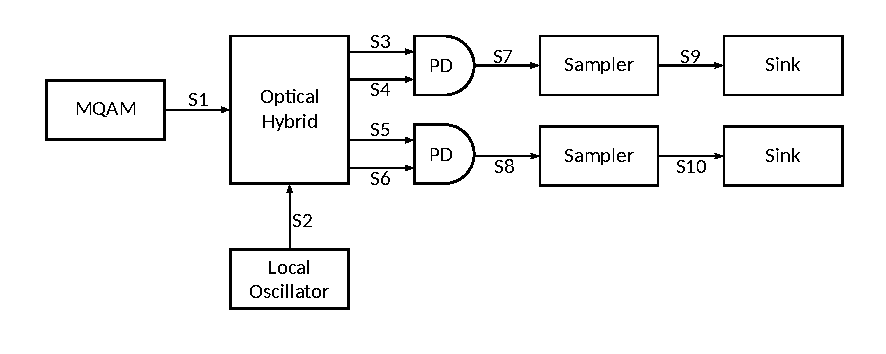
\includegraphics[width=\linewidth]{./sdf/quantum_noise/figures/scheme1.pdf}
\caption{Overview of the optical system being simulated.}
\label{fig:setup}
\end{figure}


\subsection*{Required files}\label{Required files}

Header Files
\begin{table}[H]
\centering
\begin{tabulary}{1.0\textwidth}{|L|L|}
\hline
\textbf{File}           & \textbf{Description}\\
\hline
netxpto.h               & Generic purpose simulator definitions.\\
\hline
m\_qam\_transmitter.h   & Outputs a QPSK modulated optical signal.??\\
\hline
local\_oscillator.h     & Generates continuous coherent signal.\\
\hline
optical\_hybrid.h       & ---\\
\hline
photodiode.h            & Converts two optical signals to a difference of photocurrents.??\\
\hline
sampler.h               & Samples the input signal.??\\
\hline
sink.h                  & Closes any unused signals.\\
\hline
\end{tabulary}
\end{table}
%
%
Source Files
\begin{table}[H]
\centering
\begin{tabulary}{1.0\textwidth}{|L|L|}
\hline
\textbf{File}                   & \textbf{Description}\\
\hline
netxpto.cpp                     & Generic purpose simulator definitions.\\
\hline
m\_qam\_transmitter.cpp         & Outputs a QPSK modulated optical signal.??\\
\hline
local\_oscillator.cpp           & Generates continuous coherent signal.\\
\hline
optical\_hybrid.cpp             & ---\\
\hline
photodiode.cpp                  & Converts two optical signals to a difference of photocurrents.??\\
\hline
sampler.cpp                     & Samples the input signal.??\\
\hline
sink.cpp                        & Closes any unused signals.\\
\hline
\end{tabulary}
\end{table}


\subsection*{System Input Parameters}

This system takes into account the following input parameters:
\begin{table}[H]
\centering
\begin{tabulary}{1.0\textwidth}{|C|L|}
\hline
\textbf{System Parameters} & \textbf{Description}\\
\hline
numberOfBitsGenerated   & Gives the number of bits to be simulated\\
\hline
bitPeriod               & Sets the time between adjacent bits\\
\hline
wavelength              & Sets the wavelength of the local oscillator in the MQAM????\\
\hline
samplesPerSymbol        & Establishes the number of samples each bit in the string is given\\
\hline
localOscillatorPower1   & Sets the optical power, in units of W, of the local oscillator inside the MQAM\\
\hline
localOscillatorPower2   & Sets the optical power, in units of W, of the local oscillator used for Bob's measurements\\
\hline
localOscillatorPhase    & Sets the initial phase of the local oscillator used in the detection\\
\hline
transferMatrix          & Sets the transfer matrix of the beam splitter used in the homodyne detector\\
\hline
responsivity            & Sets the responsivity of the photodiodes used in the homodyne detectors\\
\hline
bufferLength            & Sets the length of the buffer used in the signals\\
\hline
iqAmplitudeValues       & Sets the amplitude of the states used in the MQAM????\\
\hline
shotNoise               & Chooses if quantum shot noise is used in the simulation\\
\hline
samplesToSkip			& Sets the number of samples to skip when writing out some of the signal files.\\
\hline
\end{tabulary}
\end{table}		

\subsection*{Inputs}

This system takes no inputs.

\pagebreak
\subsection*{Outputs}

The system outputs the following objects:
\begin{itemize}
\item Signals:
\begin{itemize}
\item Binary Sequence used in the MQAM; (S$_{0}$)
\item Local Oscillator used in the MQAM; (S$_{1}$)
\item Local Oscillator used in the detection; (S$_{2}$)
\item Optical Hybrid Outputs; (S$_{3}$, S$_{4}$, S$_{5}$, S$_{6}$)
\item In phase Photodiode output; (S$_{7}$)
\item Quadrature Photodiode output; (S$_{8}$)
\item In phase Sampler output; (S$_{9}$)
\item Quadrature Sampler output; (S$_{10}$)
\end{itemize}
\end{itemize}	

\subsection*{Simulation Results}\label{subsec:SHresults}

The objective of this simulation was to get the (quantum noise???) associated to the detection of coherent states.\\
\\
\begin{figure}[h]
\centering
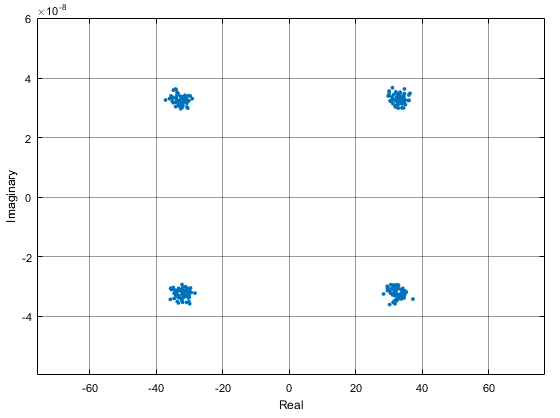
\includegraphics[width=10cm]{./sdf/quantum_noise/figures/constelation1.png}
\caption{Simulation of a constelation of 4 states (n = 100)}
\label{fig:constelation}
\end{figure}
\\
We expect that the variance is invariant with the number of photons sent from Alice. The plot in \ref{fig:variance} show that the simulation also shows this invariance with the number of photons.\\
\begin{figure}[H]
\centering
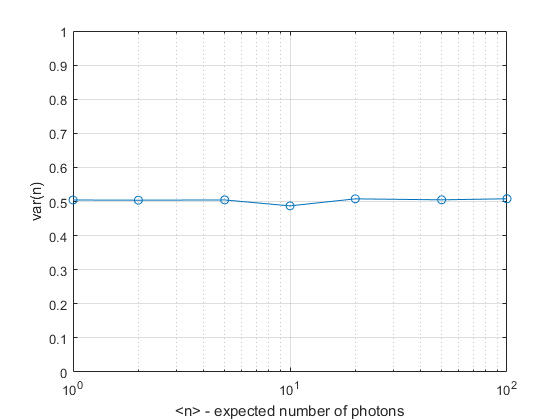
\includegraphics[width=10cm]{./sdf/quantum_noise/figures/variance_n.png}
\caption{Simulation of the variance of $n$.}
\label{fig:variance}
\end{figure}
We can conclude that the expected variance will give us $\textrm{Var(X)} = \frac{1}{2}$.\\
The results obtained in our simulations are in accordance with the theoretical prevision???


%\subsection*{Block Description}
%
%\subsubsection*{MQAM mapper???}
%\subfile{../../lib/tex/m_qam_mapper_v2}
%
%\subsection{Local Oscillator}
%\subfile{../../lib/tex/localoscillator}
%1
%\subsection{Optical Hybrid}
%MISSING FILE FOR OPTICAL HYBRID\\
%%\subfile{../../lib/tex/beamsplitter}
%
%\subsection{Photodiode}
%\subfile{../../lib/tex/photodiode}
%
%\subsection{Sampler}
%\subfile{../../lib/tex/sampler}

\subsection*{Known Problems}
\begin{enumerate}
    \item ----
\end{enumerate}

